% !TEX root = ../main.tex
\title{Synthesis-Based and Analysis-Based Hemodynamic Deconvolution for fMRI}
\label{cha:synthesis_analysis}

\begin{framed}\noindent This chapter was published as
\fullcite{Urunuela2023HemodynamicDeconvolutionDemystified}. DOI:
\url{https://doi.org/10.52294/001c.87574}.
\end{framed}

Deconvolution of the hemodynamic response is an important step to access short
timescales of brain activity recorded by functional magnetic resonance imaging
(fMRI). Albeit conventional deconvolution algorithms have been around for a long
time (e.g., Wiener deconvolution), recent state-of-the-art methods based on
sparsity-pursuing regularization are attracting increasing interest to
investigate brain dynamics and connectivity with fMRI. This chapter describes
the principles of hemodynamic deconvolution in fMRI, and revisits the main
concepts underlying two main sparsity-promoting deconvolution algorithms,
\acrlong*{pfm} and Total Activation, in an accessible manner. Despite their
apparent differences in the formulation, these methods are shown theoretically
equivalent as they represent the synthesis and analysis sides of the same
problem, respectively. This chapter demonstrates this equivalence in practice
with their best-available implementations using both simulations, with different
signal-to-noise ratios, and experimental fMRI data acquired during a motor task
and resting-state. The chapter also evaluates the parameter settings that lead
to equivalent results, and showcases the operation of these algorithms in
comparison with \acrlong*{cap} analysis. This note is useful for practitioners
interested in gaining a better understanding of state-of-the-art hemodynamic
deconvolution, and aims to answer questions regarding the differences between
the two methods.

% Introduction
\section{Introduction}
\label{sec:synthesis_introduction}

Functional magnetic resonance imaging (fMRI) data analysis is often directed to
identify and disentangle the neural processes that occur in different brain
regions during task or at rest. As the blood oxygenation level-dependent (BOLD)
signal of fMRI \citep{Ogawa1990Brainmagneticresonance} is only a proxy for
neuronal activity mediated through neurovascular coupling
\citep{Logothetis2001Neurophysiologicalinvestigationbasis}, an intermediate step
that estimates the activity-inducing signal, at the timescale of fMRI, from the
BOLD timeseries can be useful. Conventional analysis of task fMRI data relies on
the general linear models (GLM) to establish statistical parametric maps of
brain activity by regression of the empirical timecourses against hypothetical
ones built from the knowledge of the experimental paradigm
\citep{Boynton1996LinearSystemsAnalysis,Cohen1997ParametricAnalysisfMRI,Friston1998EventRelatedfMRI,Friston2008DEMvariationaltreatment}.
However, timing information of the paradigm can be unknown, inaccurate, or
insufficient in some scenarios such as naturalistic stimuli, resting-state, or
clinically-relevant assessments.

Deconvolution and methods alike are aiming to estimate neuronal activity by
undoing the blurring effect of the hemodynamic response, characterized as a
hemodynamic response function (HRF)\footnote{Note that the term deconvolution is
also alternatively employed to refer to the estimation of the hemodynamic
response shape assuming a known activity-inducing signal or neuronal activity
\citep{Goutte2000Modelinghaemodynamicresponse,Marrelec2002Bayesianestimationhemodynamic,
Ciuciu2003Unsupervisedrobustnonparametric,Casanova2008impacttemporalregularization}.
}. Given the inherently ill-posed nature of hemodynamic deconvolution, due to
the sluggish characteristics of the \acrshort*{hrf}, the key is to introduce
additional constraints in the estimation problem that are typically expressed as
regularization terms. For instance, the so-called Wiener deconvolution is
expressing a \enquote{minimal energy} constraint on the deconvolved signal, and
has been used in the framework of psychophysiological interaction analysis to
compute the interaction between a seed's activity-inducing timecourse and an
experimental modulation
\citep{Glover1999DeconvolutionImpulseResponse,Gitelman2003Modelingregionalpsychophysiologic,
Gerchen2014Analyzingtaskdependent,Di2018TaskConnectomicsExamining,
Freitas2020Timeresolvedeffective}. Complementarily, the interest in
deconvolution has increased to explore time-varying activity in resting-state
fMRI data
\citep{Preti2017dynamicfunctionalconnectome,Keilholz2017TimeResolvedResting,
Lurie2020Questionscontroversiesstudy,Bolton2020TappingMultiFaceted}. In that
case, the aim is to gain better insights of the neural signals that drive
functional connectivity at short time scales, as well as learning about the
spatio-temporal structure of functional components that dynamically construct
resting-state networks and their interactions
\citep{Karahanoglu2017Dynamicslargescale}.

Deconvolution of the resting-state fMRI signal has illustrated the significance
of transient, sparse spontaneous events
\citep{Petridou2013PeriodsrestfMRI,Allan2015FunctionalConnectivityMRI} that
refine the hierarchical clusterization of functional networks
\citep{Karahanoglu2013TotalactivationfMRI} and reveal their temporal overlap
based on their signal innovations not only in the human brain
\citep{Karahanoglu2015Transientbrainactivity}, but also in the spinal cord
\citep{Kinany2020DynamicFunctionalConnectivity}. Similar to task-related
studies, deconvolution allows to investigate modulatory interactions within and
between resting-state functional networks
\citep{Di2013ModulatoryInteractionsResting,Di2015Characterizationsrestingstate}.
In addition, decoding of the deconvolved spontaneous events allows to decipher
the flow of spontaneous thoughts and actions across different cognitive and
sensory domains while at rest
\citep{Karahanoglu2015Transientbrainactivity,GonzalezCastillo2019Imagingspontaneousflow,Tan2017DecodingfMRIevents}.
Beyond findings on healthy subjects, deconvolution techniques have also proven
its utility in clinical conditions to characterize functional alterations of
patients with a progressive stage of multiple sclerosis at rest
\citep{Bommarito2021Alteredanteriordefault}, to find functional signatures of
prodromal psychotic symptoms and anxiety at rest on patients suffering from
schizophrenia \citep{Zoeller2019LargeScaleBrain}, to detect the foci of
interictal events in epilepsy patients without an EEG recording
\citep{Lopes2012Detectionepilepticactivity,Karahanoglu2013Spatialmappinginterictal},
or to study functional dissociations observed during non-rapid eye movement
sleep that are associated with reduced consolidation of information and impaired
consciousness \citep{Tarun2021NREMsleepstages}.

The algorithms for hemodynamic deconvolution can be classified based on the
assumed hemodynamic model and the optimization problem used to estimate the
neuronal-related signal. Most approaches assume a linear time-invariant model
for the hemodynamic response that is inverted by means of variational
(regularized) least squares estimators
\citep{Glover1999DeconvolutionImpulseResponse,Gitelman2003Modelingregionalpsychophysiologic,
Gaudes2010Detectioncharacterizationsingle,Gaudes2012Structuredsparsedeconvolution,
Gaudes2013Paradigmfreemapping,CaballeroGaudes2019deconvolutionalgorithmmulti,
HernandezGarcia2011Neuronaleventdetection,Karahanoglu2013TotalactivationfMRI,
Cherkaoui2019Sparsitybasedblind,
Huetel2021Hemodynamicmatrixfactorization,Costantini2022Anisotropic4DFiltering},
logistic functions
\citep{Bush2013Decodingneuralevents,Bush2015deconvolutionbasedapproach,
Loula2018DecodingfMRIactivity}, probabilistic mixture models
\citep{Pidnebesna2019EstimatingSparseNeuronal}, convolutional autoencoders
\citep{Huetel2018NeuralActivationEstimation} or nonparametric homomorphic
filtering \citep{Sreenivasan2015NonparametricHemodynamicDeconvolution}.
Alternatively, several methods have also been proposed to invert non-linear
models of the neuronal and hemodynamic coupling
\citep{Riera2004statespacemodel,Penny2005Bilineardynamicalsystems,Friston2008DEMvariationaltreatment,
Havlicek2011Dynamicmodelingneuronal,Aslan2016Jointstateparameter,
Madi2017HybridCubatureKalman,RuizEuler2018NonlinearDeconvolutionSampling}.

Among the variety of approaches, those based on regularized least squares
estimators have been employed more often due to their appropriate performance at
small spatial scales (e.g., voxelwise). Relevant for this work, two different
formulations can be established for the regularized least-squares deconvolution
problem, either based on a synthesis- or analysis-based model
\citep{Elad2007Analysisversussynthesis,Ortelli2019Synthesisanalysistotal}. On
the one hand, \acrlong*{pfm} is based on a synthesis formulation that is solved
by means of regularized least-squares estimators such as ridge-regression
\citep{Gaudes2010Detectioncharacterizationsingle} or LASSO
\citep{Gaudes2013Paradigmfreemapping}. The rationale of the synthesis-based
model is that we know or suspect that the true signal (here, the
neuronally-driven BOLD component of the fMRI signal) can be represented as a
linear combination of predefined patterns or dictionary atoms (for instance, the
hemodynamic response function). On the other hand, Total Activation is based on
a analysis formulation that is solved with a regularized least-squares estimator
using generalized total variation
\citep{Karahanoglu2011SignalProcessingApproach,Karahanoglu2013TotalactivationfMRI}.
The rationale of the analysis-based approach considers that the true signal is
analyzed by some relevant hemodynamic operator
\citep{Khalidov2011ActiveletsWaveletssparse} and the resulting signal is sparse
in time.

The users of these algorithms have often questioned about the similarities and
differences between the two methods and which one is better. To clarify this
point, this chapter initially presents the theory behind these two deconvolution
approaches: \acrfull*{pfm} \citep{Gaudes2013Paradigmfreemapping} --- available
in AFNI as
\textit{3dPFM}\footnote{\url{https://afni.nimh.nih.gov/pub/dist/doc/program_help/3dPFM.html}}
and
\textit{3dMEPFM}\footnote{\url{https://afni.nimh.nih.gov/pub/dist/doc/program_help/3dMEPFM.html}}
for single-echo and multi-echo data, respectively --- and \acrfull*{ta}
\citep{Karahanoglu2013TotalactivationfMRI} --- available as part of the
\textit{iCAPs toolbox}\footnote{\url{https://c4science.ch/source/iCAPs/}}. The
chapter describes the similarities and differences in their analytical
formulations, and how they can be related to each other. Next, their performance
is assessed controlling for a fair comparison on simulated and experimental
data. Finally, the chapter discusses their benefits and shortcomings and
conclude with our vision on potential extensions and developments.

% Theory
\section{Theory}
\label{sec:synthesis_theory}
\subsection{Notations and Definitions}

Matrices of size $N$ rows and $M$ columns are denoted by boldface capital
letters, e.g., $\mathbf{X} \in \mathbb{R}^{N\times M}$, whereas column vectors
of length $N$ are denoted as boldface lowercase letters, e.g., $\mathbf{x} \in
\mathbb{R}^{N}$. Scalars are denoted by lowercase letters, e.g., $k$. Continuous
functions are denoted by brackets, e.g., $h(t)$, while discrete functions are
denoted by square brackets, e.g., $x[k]$. The Euclidean norm of a matrix
$\mathbf{X}$ is denoted as $\|\mathbf{X}\|_2$, the $\ell_1$-norm is denoted by
$\| \mathbf{X} \|_1$ and the Frobenius norm is denoted by $\| \mathbf{X} \|_F$.
The discrete integration ($\mathbf{L}$) and difference ($\mathbf{D}$) operators
are defined as:

$$
\mathbf{L} = \left[\begin{array}{ccccc}
1 & 0 & \ldots & & \\
1 & 1 & 0 & \ldots & \\
1 & 1 & 1 & 0 & \ldots \\
\vdots & \ddots & \ddots & \ddots & \ddots
\end{array}\right], \quad \mathbf{D} = \left[\begin{array}{ccccc}
1 & 0 & \ldots & & \\
1 & -1 & 0 & \ldots & \\
0 & \ddots & \ddots & \ddots & \ldots \\
\vdots & \ddots & 0 & 1 & -1
\end{array}\right].
$$

\subsection{General Linear Model Analysis}

A conventional general linear model (GLM) analysis puts forward a number of
regressors incorporating the knowledge about the paradigm or behavior. For
instance, the timing of epochs for a certain condition can be modeled as an
indicator function $p(t)$ (e.g., Dirac functions for event-related designs or
box-car functions for block-designs) convolved with the hemodynamic response
function (HRF) $h(t)$, and sampled at the repetition time (TR) resolution
\citep{Friston1994AnalysisfunctionalMRI,Friston1998EventRelatedfMRI,
Boynton1996LinearSystemsAnalysis,Cohen1997ParametricAnalysisfMRI}:
$$
   x(t) = p*h(t) \rightarrow x[k] = p*h(k\cdot\text{TR}).
$$
The vector $\mathbf{x}=[x[k]]_{k=1,\ldots,N} \in \mathbb{R}^{N}$ then
constitutes the regressor modelling the hypothetical response, and several of
them can be stacked as columns of the design matrix $\mathbf{X}=[\mathbf{x}_1
\ldots \mathbf{x}_L] \in \mathbb{R}^{N \times L}$, leading to the well-known GLM
formulation:
\begin{equation}
    \label{eq:glm}
    \mathbf{y} = \mathbf{X} \boldsymbol\beta + \mathbf{e},
\end{equation}
where the empirical timecourse $\mathbf{y} \in \mathbb{R}^{N}$ is explained by a
linear combination of the regressors in $\mathbf{X}$ weighted by the parameters
in $\boldsymbol\beta \in \mathbb{R}^{L}$ and corrupted by additive noise
$\mathbf{e}\in \mathbb{R}^{N}$. Under independent and identically distributed
Gaussian assumptions of the latter, the maximum likelihood estimate of the
parameter weights reverts to the ordinary least-squares estimator; i.e.,
minimizing the residual sum of squares between the fitted model and
measurements. The number of regressors $L$ is typically much less than the
number of measurements $N$, and thus the regression problem is over-determined
and does not require additional constraints or assumptions
\citep{Henson2007CHAPTER14Convolution}.

In the deconvolution approach, no prior knowledge of the hypothetical response
is taken into account, and the purpose is to estimate the deconvolved
activity-inducing signal $\mathbf{s}$ from the measurements $\mathbf{y}$, which
can be formulated as the following signal model
\begin{equation}
    \label{eq:synthesis_model}
    \mathbf{y} = \mathbf{Hs} + \mathbf{e},
\end{equation}
where $\mathbf{H} \in \mathbb{R}^{N \times N}$ is a Toeplitz matrix that
represents the discrete convolution with the HRF, and $\mathbf{s} \in
\mathbb{R}^{N}$ is a length-$N$ vector with the unknown activity-inducing
signal. Note that the temporal resolution of the activity-inducing signal and
the corresponding Toeplitz matrix is generally assumed to be equal to the TR of
the acquisition, but it could also be higher if an upsampled estimate is
desired. Despite the apparent similarity with the GLM equation, there are two
important differences. First, the multiplication with the design matrix of the
GLM is an expansion as a weighted linear combination of its columns, while the
multiplication with the HRF matrix represents a convolution operator. Second,
determining $\mathbf{s}$ is an ill-posed problem given the nature of the HRF. As
it can be seen intuitively, the convolution matrix $\mathbf{H}$ is highly
collinear (i.e., its columns are highly correlated) due to large overlap between
shifted HRFs (see \cref{fig:sim_and_hrf}C), thus introducing uncertainty in the
estimates of $\mathbf{s}$ when noise is present. Consequently, additional
assumptions under the form of regularization terms (or priors) in the estimate
are needed to reduce their variance. In the least squares sense, the
optimization problem to solve is given by
\begin{equation}
    \label{eq:regularized_least_squares}
    \hat{\mathbf{s}} = \arg \min_{\mathbf{s}} \frac{1}{2} \| \mathbf{y} - \mathbf{Hs} \|_2^2 + \Omega(\mathbf{s}).
\end{equation}
The first term quantifies data fitness, which can be justified as the
log-likelihood term derived from Gaussian noise assumptions, while the second
term \(\Omega(\mathbf{s})\) brings in regularization and can be interpreted as a
prior on the activity-inducing signal. For example, the $\ell_2$-norm of
$\mathbf{s}$ (i.e., $\Omega(\mathbf{s})=\lambda \left\| \mathbf{s}\right\|_2^2$)
is imposed for ridge regression or Wiener deconvolution, which introduces a
trade-off between the data fit term and \enquote{energy} of the estimates that
is controlled by the regularization parameter $\lambda$. Other well-known
regularized terms are related to the elastic net (i.e.,
$\Omega(\mathbf{x})=\lambda_1\|\mathbf{x}\|_2^2 + \lambda_2\|\mathbf{x}\|_1$)
\citep{Zou2005Regularizationvariableselection}.

%%%%%%%%%%%%%%%%%%%%%%%%%%%%%%%%%%%%%%%%%%%%%%%%%%%%%%%%%%%%%%%%%%%%%%%%
% \acrlong*{pfm}
%%%%%%%%%%%%%%%%%%%%%%%%%%%%%%%%%%%%%%%%%%%%%%%%%%%%%%%%%%%%%%%%%%%%%%%%

\subsection{\acrlong*{pfm}} In \acrfull*{pfm}, the formulation of
\cref{eq:regularized_least_squares} was considered equivalently as fitting the
measurements using the atoms of the HRF dictionary (i.e., columns of
$\mathbf{H}$) with corresponding weights (entries of $\mathbf{s}$). This model
corresponds to a synthesis formulation. In \cite{Gaudes2013Paradigmfreemapping}
a sparsity-pursuing regularization term was introduced on $\mathbf{s}$, which in
a strict way reverts to choosing \(\Omega(\mathbf{s})=\lambda \| \mathbf{s}
\|_0\) as the regularization term and solving the optimization problem
\citep{Bruckstein2009SparseSolutionsSystems}. However, finding the optimal
solution to the problem demands an exhaustive search across all possible
combinations of the columns of \(\mathbf{H}\). Hence, a  pragmatic solution is
to solve the convex-relaxed optimization problem for the \(l_1\)-norm, commonly
known as Basis Pursuit Denoising \citep{Chen2001Atomicdecompositionbasis} or
equivalently as the least absolute shrinkage and selection operator (LASSO)
\citep{Tibshirani1996RegressionShrinkageSelection}:
\begin{equation}
    \label{eq:pfm_spike}
    \hat{\mathbf{s}} = \arg \min_{\mathbf{s}} \frac{1}{2} \| \mathbf{y} - \mathbf{Hs} \|_2^2 + \lambda \| \mathbf{s} \|_1,
\end{equation}
which provides fast convergence to a global solution. Imposing sparsity on the
activity-inducing signal implies that it is assumed to be well represented by a
reduced subset of few non-zero coefficients at the fMRI timescale, which in turn
trigger event-related BOLD responses. Hereinafter, this assumption is referred
to as the \textit{spike model}. However, even if PFM was developed as a spike
model, its formulation in \cref{eq:pfm_spike} can be extended to estimate the
innovation signal, i.e., the derivative of the activity-inducing signal, as
shown in \cref{sec:unifying_both_perspectives}.

%%%%%%%%%%%%%%%%%%%%%%%%%%%%%%%%%%%%%%%%%%%%%%%%%%%%%%%%%%%%%%%%%%%%%%%%
% Total Activation
%%%%%%%%%%%%%%%%%%%%%%%%%%%%%%%%%%%%%%%%%%%%%%%%%%%%%%%%%%%%%%%%%%%%%%%%

\subsection{Total Activation}
Alternatively, deconvolution can be formulated as if the signal to be recovered
directly fits the measurements and at the same time satisfies some suitable
regularization, which leads to
\begin{equation}
\label{eq:analysis_model}
    \hat{\mathbf{x}} = \arg \min_{\mathbf{x}} \frac{1}{2} \| \mathbf{y} - \mathbf{x} \|_2^2 + \Omega(\mathbf{x}).
\end{equation}
Under this analysis formulation, total variation (TV), i.e., the $\ell_1$-norm
of the derivative $\Omega(\mathbf{x})=\lambda \|\mathbf{Dx}\|_1$, is a powerful
regularizer since it favors recovery of piecewise-constant signals
\citep{Chambolle2004algorithmtotalvariation}. Going beyond, the approach of
generalized TV introduces an additional differential operator $\mathbf{D_H}$ in
the regularizer that can be tailored as the inverse operator of a linear system
\citep{Karahanoglu2011SignalProcessingApproach}, that is,
$\Omega(\mathbf{x})=\lambda \|\mathbf{D D_H x}\|_1$. In the context of
hemodynamic deconvolution, Total Activation is proposed for which the discrete
operator $\mathbf{D_H}$ is derived from the inverse of the continuous-domain
linearized Balloon-Windkessel model
\citep{Buxton1998Dynamicsbloodflow,Friston2000NonlinearresponsesfMRI}. The
interested reader is referred to
\citep{Khalidov2011ActiveletsWaveletssparse,Karahanoglu2011SignalProcessingApproach,Karahanoglu2013TotalactivationfMRI}
for a detailed description of this derivation.

Therefore, the solution of the Total Activation (TA) problem
\begin{equation}
\label{eq:TA}
    \hat{\mathbf{x}} = \arg \min_{\mathbf{x}} \frac{1}{2} \| \mathbf{y} - \mathbf{x} \|_2^2 + \lambda \|\mathbf{D D_H x} \|_1
\end{equation}
will yield the activity-related signal $\mathbf{x}$ for which the
activity-inducing signal $\mathbf{s}=\mathbf{D_H x}$ and the so-called
innovation signal $\mathbf{u}=\mathbf{Ds}$, i.e., the derivate of the
activity-inducing signal, will also be available, as they are required for the
regularization. Modeling the activity-inducing signal based on the innovation
signal is referred to as the \textit{block model}. Nevertheless, even if TA was
originally developed as a block model, its formulation in \cref{eq:TA} can be
made equivalent to the spike model as shown in
\cref{sec:unifying_both_perspectives}.

\subsection{Unifying Both Perspectives}
\label{sec:unifying_both_perspectives}
PFM and TA are based on the synthesis- and analysis-based formulation of the
deconvolution problem, respectively. They are also tailored for the spike and
block model, respectively. In the first case, the recovered deconvolved signal
is synthesized to be matched to the measurements, while in the second case, the
recovered signal is directly matched to the measurements but needs to satisfy
its analysis in terms of deconvolution. This also corresponds to using the
forward or backward model of the hemodynamic system, respectively. Hence, it is
possible to make both approaches equivalent
\citep{Elad2007Analysisversussynthesis}\footnote{Without dwelling into
technicalities, for total variation, this equivalence is correct up to the
constant, which is in the null space of the derivative operator.}.

To start with, TA can be made equivalent to PFM by adapting it for the spike
model; i.e., when removing the derivative operator $\mathbf{D}$ of the
regularizer in \cref{eq:TA}, it can be readily verified that replacing in that
case $\mathbf{x}=\mathbf{Hs}$ leads to identical equations and thus both assume
a spike model, since $\mathbf{H}$ and $\mathbf{D_H}$ will cancel out each other
\citep{Karahanoglu2011SignalProcessingApproach}\footnote{Again, this holds up to
elements of the null space.}.

Conversely, the PFM spike model can also accommodate the TA block model by
modifying \cref{eq:pfm_spike} with the forward model $\mathbf{y} = \mathbf{H L
u} + \mathbf{e}$. Here, the activity-inducing signal $\mathbf{s}$ is rewritten
in terms of the innovation signal $\mathbf{u}$ as $\mathbf{s}=\mathbf{Lu}$ where
the matrix $\mathbf{L}$ is the first-order integration operator
\citep{Cherkaoui2019Sparsitybasedblind,Urunuela2020StabilityBasedSparse}. This
way, PFM can estimate the innovation signal $\mathbf{u}$ as follows:
\begin{equation}
    \label{eq:pfm_block}
    \hat{\mathbf{u}} = \arg \min_{\mathbf{u}} \frac{1}{2} \| \mathbf{y} - \mathbf{HLu} \|_2^2 + \lambda \| \mathbf{u} \|_1,
\end{equation}
and becomes equivalent to TA by replacing $\mathbf{u}=\mathbf{D D_H x}$, and
thus adopting the block model. Based on the previous equations
(\cref{eq:pfm_spike}), (\cref{eq:TA}) and (\cref{eq:pfm_block}), it is clear
that both PFM and TA can operate under the spike and block models, providing a
convenient signal model according to the different assumptions of the underlying
neuronal-related signal. This work evaluates the core of the two techniques;
i.e., the regularized least-squares problem with temporal regularization without
considering the spatial regularization term originally incorporated in TA. For
the remainder of this paper, the PFM and TA formalisms with both spike and block
models are used.

\begin{figure}[t!]
    \begin{center}
        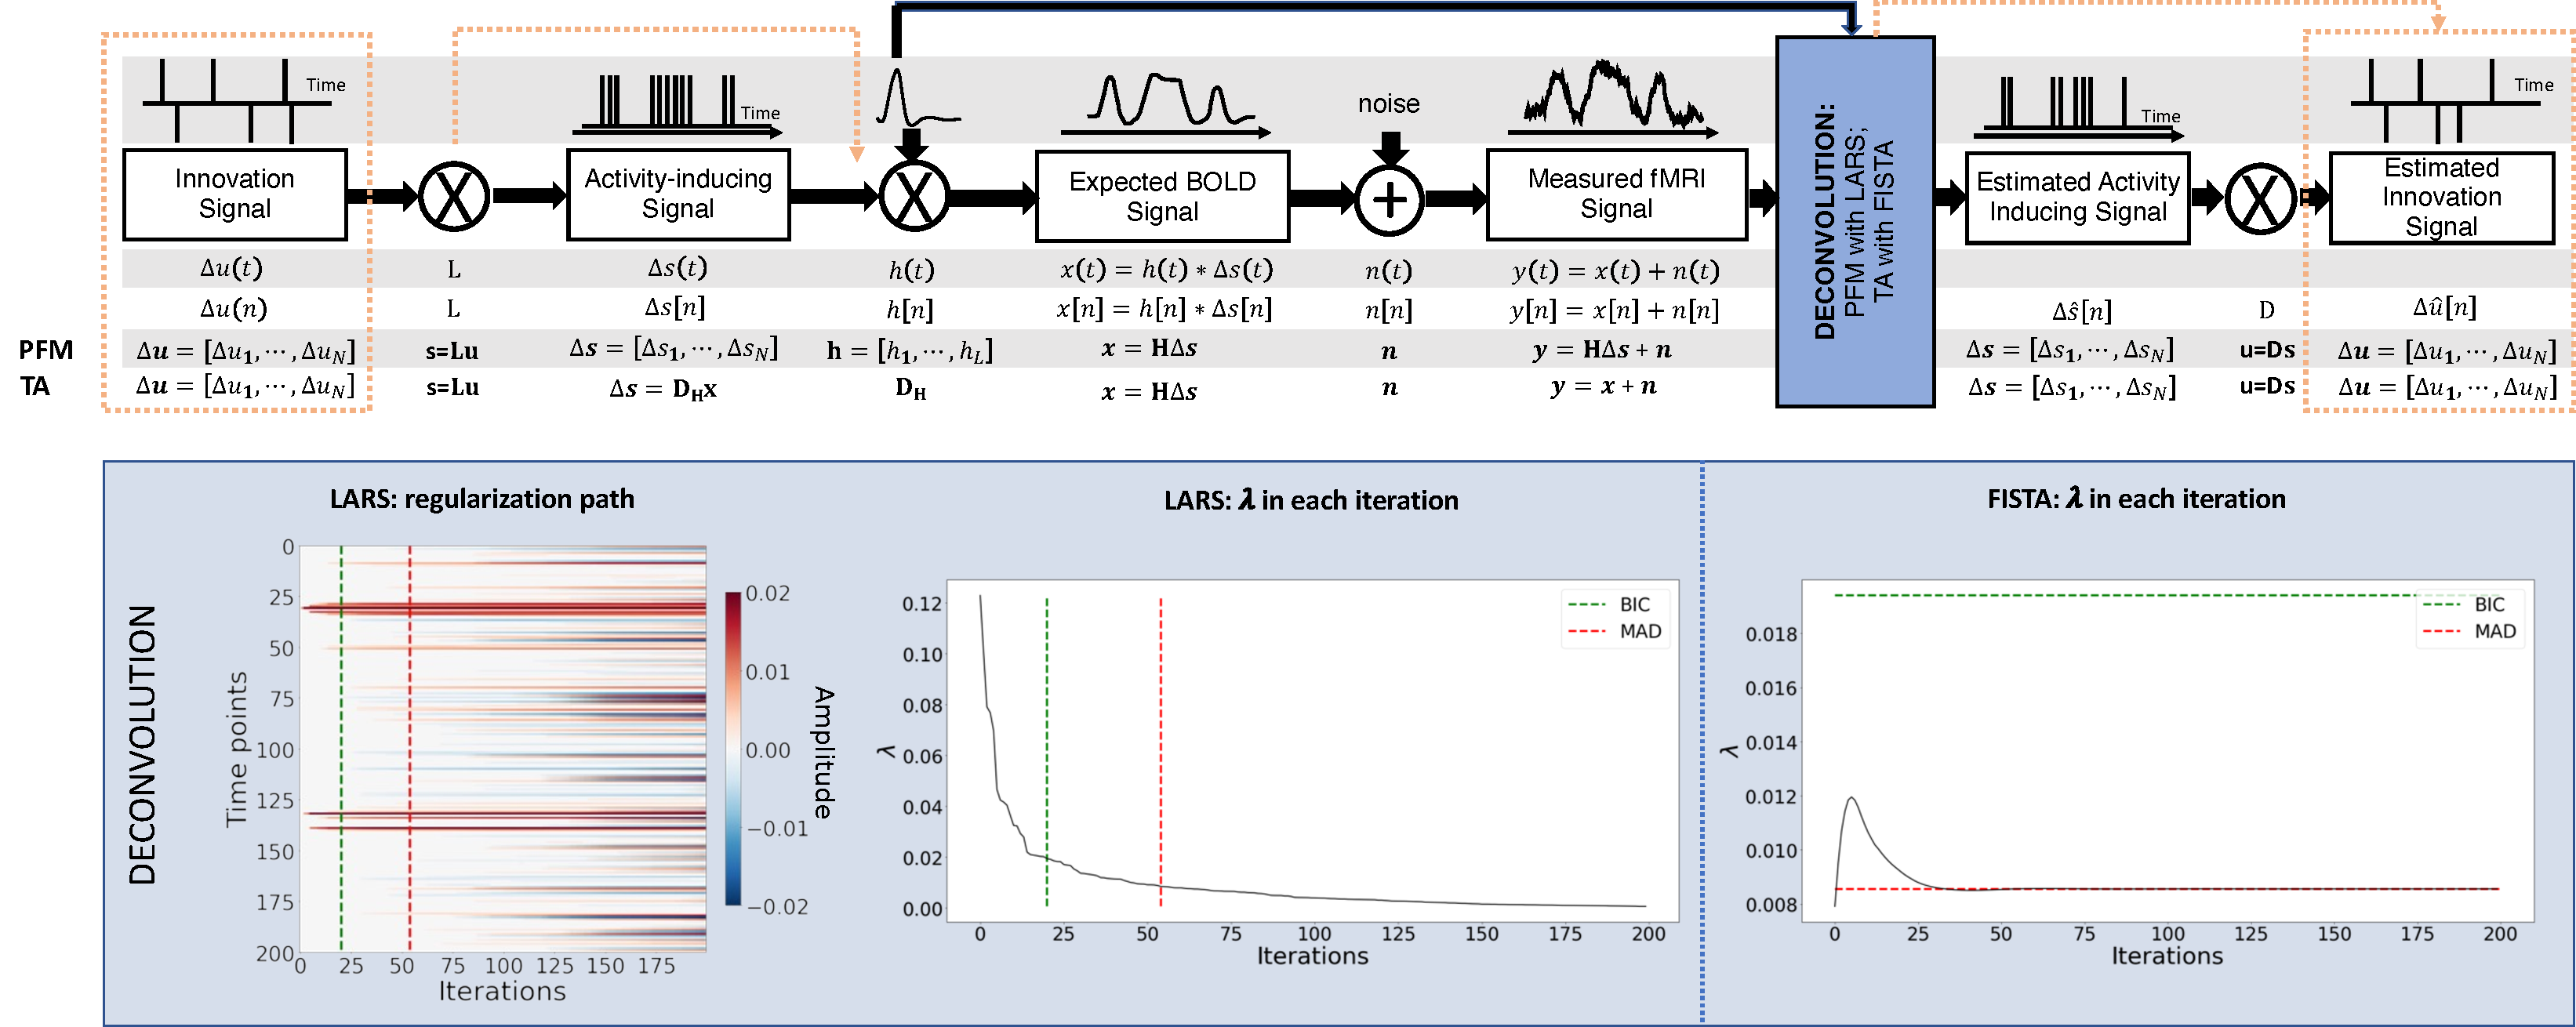
\includegraphics[width=\textwidth]{figures/synthesis_analysis/flowchart.pdf}
    \end{center}
    \caption{Flowchart detailing the different steps of the fMRI signal and the
    deconvolution methods described. The orange arrows indicate the flow to
    estimate the innovation signals, i.e., the derivative of the
    activity-inducing signal. The blue box depicts the iterative \textit{modus
    operandi} of the two algorithms used in this paper to solve the paradigm
    free mapping (PFM) and \acrfull*{ta} deconvolution problems. The plot on the
    left shows the regularization path obtained with the least angle regression
    (LARS) algorithm, where the x-axis illustrates the different iterations of
    the algorithm, the y-axis represents points in time, and the color describes
    the amplitude of the estimated signal. The middle plot depicts the
    decreasing values of $\lambda$ for each iteration of LARS as the
    regularization path is computed. The green and red dashed lines in both
    plots illustrate the Bayesian information criterion (BIC) and median
    absolute deviation (MAD) solutions, respectively. Comparatively, the changes
    in $\lambda$ when the fast iterative shrinkage-thresholding algorithm
    (FISTA) method is made to converge to the MAD estimate of the noise are
    shown on the right. Likewise, the $\lambda$ corresponding to the BIC and MAD
    solutions are shown with dashed lines.}
\label{fig:flowchart}
\end{figure}

\subsection{Algorithms and Parameter Selection}
\label{sec:regparam}
Despite their apparent resemblance, the practical implementations of the PFM and
TA methods proposed different algorithms to solve the corresponding optimization
problem and select an adequate regularization parameter $\lambda$
\citep{Gaudes2013Paradigmfreemapping,Karahanoglu2013TotalactivationfMRI}. The
PFM implementation available in AFNI employs the least angle regression (LARS)
\citep{Efron2004Leastangleregression}, whereas the TA implementation uses the
fast iterative shrinkage-thresholding algorithm (FISTA)
\citep{Beck2009FastIterativeShrinkage}. The blue box in \cref{fig:flowchart}
provides a descriptive view of the iterative \textit{modus operandi} of the two
algorithms.

On the one hand, LARS is a homotopy approach that computes all the possible
solutions to the optimization problem and their corresponding value of
$\lambda$; i.e., the regularization path, and the solution according to the
Bayesian Information Criterion (BIC)
\citep{Schwarz1978EstimatingDimensionModel}, was recommended as the most
appropriate in the case of PFM approaches since Akaike Information Criterion
(AIC) often tends to overfit the signal
\citep{Gaudes2013Paradigmfreemapping,CaballeroGaudes2019deconvolutionalgorithmmulti}.

On the other hand, FISTA is an extension of the classical gradient algorithm
that provides fast convergence for large-scale problems. In the case of FISTA
though, the regularization parameter $\lambda$ must be selected prior to solving
the problem, but can be updated in every iteration so that the residuals of the
data fit converge to an estimated noise level of the data $\hat{\sigma}$:
\begin{equation}
    \lambda^{n+1} = \frac{N \hat{\sigma}}{\frac{1}{2} \| \mathbf{y} - \mathbf{x}^n \|_F^2} \lambda^n,
\label{eq:std}
\end{equation}
where $x^n$ is the $n^{th}$ iteration estimate, $\lambda^n$ and $\lambda^{n+1}$
are the $n^{th}$ and $n+1^{th}$ iteration values for the regularization
parameter $\lambda$, and $N$ is the number of points in the time-course. The
pre-estimated noise level can be obtained as the median absolute deviation (MAD)
of the fine-scale wavelet coefficients (Daubechies, order 3) of the fMRI
timecourse. The MAD criterion has been adopted in TA
\citep{Karahanoglu2013TotalactivationfMRI}. Of note, similar formulations based
on the MAD estimate have also been applied in PFM formulations
\citep{Gaudes2012Structuredsparsedeconvolution,Gaudes2011Paradigmfreemapping}.

% Methods
\section{Methods}
\label{sec:synthesis_methods}

\subsection{Simulated data}

\begin{figure}[t!]
    \begin{center}
        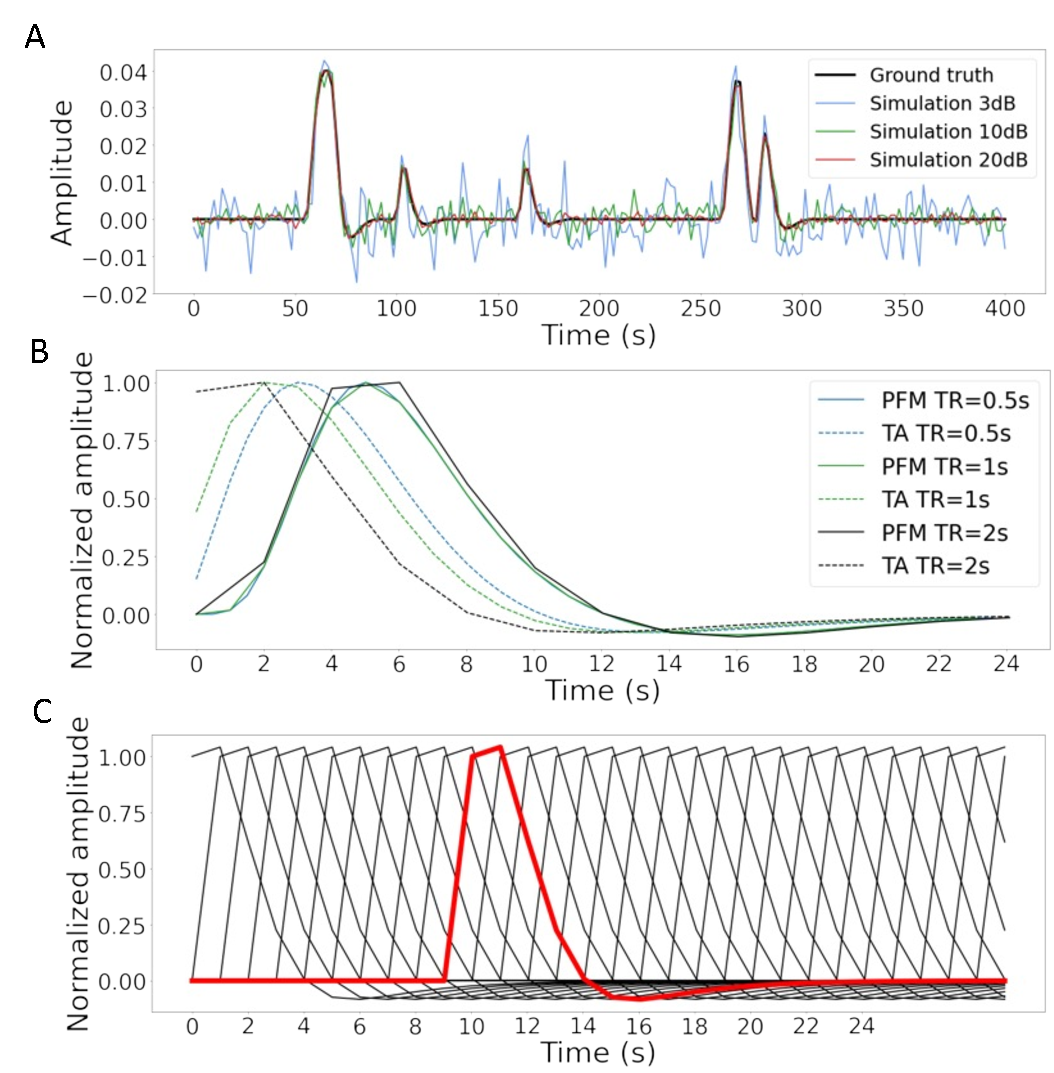
\includegraphics[width=0.75\columnwidth]{figures/synthesis_analysis/sim_and_hrf.pdf}
    \end{center}
    \caption{A) Simulated signal with different SNRs (20 dB, 10 dB and 3 dB) and ground truth given in signal percentage change (SPC). B) Canonical HRF models typically used by PFM (solid line) and TA (dashed line) at TR = 0.5 s (blue), TR = 1 s (green) and TR = 2 s (black). Without loss of generality, the waveforms are scaled to unit amplitude for visualization. C) Representation of shifted HRFs at TR = 2 s that build the design matrix for PFM when the HRF model has been matched to that in TA. The red line corresponds to one of the columns of the HRF matrix.}
\label{fig:sim_and_hrf}
\end{figure}

In order to compare the two methods while controlling for their correct
performance, a simulation scenario was created, which can be found in the GitHub
repository shared in \cref{sec:synthesis_github}. For the sake of illustration,
here the simulations correspond to a timecourse with a duration of 400 seconds
(TR = 2 s) where the activity-inducing signal includes 5 events, which are
convolved with the canonical HRF. Different noise sources (physiological,
thermal, and motion-related) were also added and three different scenarios with
varying signal-to-noise ratios (SNR = 20, 10, 3 dB) were simulated, which
represent high, medium and low contrast-to-noise ratios as shown in
\cref{fig:sim_and_hrf}A. Noise was created following the procedure in
\citep{Gaudes2013Paradigmfreemapping} as the sum of uncorrelated Gaussian noise
and sinusoidal signals to simulate a realistic noise model with thermal noise,
cardiac and respiratory physiological fluctuations, respectively. The
physiological signals were generated as
\begin{equation}
    \sum_{i=1}^{2} \frac{1}{2^{i-1}}\left(\sin \left(2 \pi f_{r, i} t+\phi_{\mathrm{r}, i}\right)+\sin \left(2 \pi f_{c, i} t+\phi_{c, i}\right)\right),
\end{equation}
with up to second-order harmonics per cardiac (\(f_{c,i}\)) and respiratory
(\(f_{r,i}\)) component that were randomly generated following normal
distributions with variance 0.04 and mean \(if_r\) and \(if_c\), for \(i = [1,
2]\). The fundamental frequencies were set to \(f_r = 0.3\) Hz for the
respiratory component \citep{Birn2006Separatingrespiratoryvariation} and \(f_c =
1.1\) Hz for the cardiac component \citep{Shmueli2007Lowfrequencyfluctuations}.
The phases of each harmonic \(\phi\) were randomly selected from a uniform
distribution between 0 and 2$\pi$ radians. To simulate physiological noise that
is proportional to the change in BOLD signal, a variable ratio between the
physiological (\(\sigma_P\)) and the thermal (\(\sigma_0\)) noise was modeled as
\(\sigma_P/\sigma_0 = a(tSNR)^b + c\), where \(a = 5.01 \times 10^{-6}\), \(b =
2.81\), and \(c = 0.397\), following the experimental measures available in
Table 3 from \citep{Triantafyllou2005Comparisonphysiologicalnoise}).

%%%%%%%%%%%%%%%%%%%%%%%%%%%%%%%%%%%%%%%%%%%%%%%%%%%%%%%%%%%
%%%%%%%%%%%%%%%%%%%%%%%%%%%%%%%%%%%%%%%%%%%%%%%%%%%%%%%%%%%
%%%%%%%%%%%%%%%%%%%%%%%%%%%%%%%%%%%%%%%%%%%%%%%%%%%%%%%%%%%
\subsection{Experimental Data}
To compare the performance of the two approaches as well as illustrate their
operation, two representative experimental datasets were employed.

\textbf{Motor task dataset:} One healthy subject was scanned in a 3T
\acrshort*{mr} scanner (Siemens) under a Basque Center on Cognition, Brain and
Language Review Board-approved protocol. T2*-weighted multi-echo fMRI data was
acquired with a simultaneous-multislice multi-echo gradient echo-planar imaging
sequence, kindly provided by the Center of Magnetic Resonance Research
(University of Minnesota, USA)
\citep{Feinberg2010MultiplexedEchoPlanar,Moeller2010MultibandmultisliceGE,Setsompop2011Blippedcontrolledaliasing},
with the following parameters: 340 time frames, 52 slices, Partial-Fourier =
6/8, voxel size = $2.4\times2.4\times3$ mm\textsuperscript{3}, TR = 1.5 s, TEs =
10.6/28.69/46.78/64.87/82.96 ms, flip angle = 70\(^o\), multiband factor = 4,
GRAPPA = 2.

During the fMRI acquisition, the subject performed a motor task consisting of
five different movements (left-hand finger tapping, right-hand finger tapping,
moving the left toes, moving the right toes and moving the tongue) that were
visually cued through a mirror located on the head coil. These conditions were
randomly intermixed every 16 seconds, and were only repeated once the entire set
of stimuli were presented. Data preprocessing consisted of first, discarding the
first 10 volumes of the functional data to achieve a steady state of
magnetization. Then, image realignment to the skull-stripped single-band
reference image (SBRef) was computed on the first echo, and the estimated
rigid-body spatial transformation was applied to all other echoes
\citep{Jenkinson2012FSL,Jenkinson2001globaloptimisationmethod}. A brain mask
obtained from the SBRef volume was applied to all the echoes and the different
echo timeseries were optimally combined (OC) voxelwise by weighting each
timeseries contribution by its T2* value
\citep{Posse1999EnhancementBOLDcontrast}. AFNI
\citep{Cox1996AFNISoftwareAnalysis} was employed for a detrending of up to
4\textsuperscript{th}-order Legendre polynomials, within-brain spatial smoothing
(3 mm FWHM) and voxelwise signal normalization to percentage change. Finally,
distortion field correction was performed on the OC volume with Topup
\citep{Andersson2003Howcorrectsusceptibility}, using the pair of spin-echo EPI
images with reversed phase encoding acquired before the ME-EPI acquisition
\citep{Glasser2016HumanConnectomeProjects}.

\textbf{Resting-state datasets:} One healthy subject was scanned in a 3T MR
scanner (Siemens) under a Basque Center on Cognition, Brain and Language Review
Board-approved protocol. Two runs of T2*-weighted fMRI data were acquired during
resting-state, each with 10 min duration, with 1) a standard gradient-echo
echo-planar imaging sequence (monoband) (TR = 2000 ms, TE = 29 ms, flip-angle =
78\(^o\), matrix size = $64\times64$, voxel size = $3\times3\times3$
mm\textsuperscript{3}, 33 axial slices with interleaved acquisition, slice gap =
0.6 mm) and 2) a  simultaneous-multislice gradient-echo echo-planar imaging
sequence (multiband factor = 3, TR = 800 ms, TE = 29 ms, flip-angle = 60\(^o\),
matrix size = $64\times64$, voxel size = $3\times3\times3$
mm\textsuperscript{3}, 42 axial slices with interleaved acquisition, no slice
gap). Single-band reference images were also collected in both resting-state
acquisitions for head motion realignment. Field maps were also obtained to
correct for field distortions.

During both acquisitions, participants were instructed to keep their eyes open,
fixating a white cross that they saw through a mirror located on the head coil,
and not to think about anything specific. The data was pre-processed using AFNI
\citep{Cox1996AFNISoftwareAnalysis}. First, volumes corresponding to the initial
10 seconds were removed to allow for a steady-state magnetization. Then, the
voxel time-series were despiked to reduce large-amplitude deviations and
slice-time corrected. Inhomogeneities caused by magnetic susceptibility were
corrected with FUGUE (FSL) using the field map images \citep{Jenkinson2012FSL}.
Next, functional images were realigned to a base volume (monoband: volume with
the lowest head motion; multiband: single-band reference image). Finally, a
simultaneous nuisance regression step was performed comprising up to
6\textsuperscript{th}-order Legendre polynomials, low-pass filtering with a
cutoff frequency of 0.25 Hz (only on multiband data to match the frequency
content of the monoband), 6 realignment parameters plus temporal derivatives, 5
principal components of white matter (WM), 5 principal components of lateral
ventricle voxels (anatomical CompCor) \citep{Behzadi2007componentbasednoise} and
5 principal components of the brain's edge voxels
\citep{Patriat2015UsingEdgeVoxel}. WM, cerebrospinal fluid (CSF) and brain's
edge-voxel masks were obtained from Freesurfer tissue and brain segmentations.
In addition, scans with potential artifacts were identified and censored when
the euclidean norm of the temporal derivative of the realignment parameters
(ENORM) was larger than 0.4, and the proportion of voxels adjusted in the
despiking step exceeded 10\%.

%%%%%%%%%%%%%%%%%%%%%%%%%%%%%%%%%%%%%%%%%%%%%%%%%%%%%%%%%%%
%%%%%%%%%%%%%%%%%%%%%%%%%%%%%%%%%%%%%%%%%%%%%%%%%%%%%%%%%%%
%%%%%%%%%%%%%%%%%%%%%%%%%%%%%%%%%%%%%%%%%%%%%%%%%%%%%%%%%%%
\subsection{Selection of the Hemodynamic Response Function}

In their original formulations, PFM and TA specify the discrete-time HRF in
different ways. For PFM, the continuous-domain specification of the canonical
double-gamma HRF \citep{Henson2007CHAPTER14Convolution} is sampled at the TR and
then put as shifted impulse responses to build the matrix $\mathbf{H}$.  In the
case of TA, however, the continuous-domain linearized version of the
balloon-windkessel model is discretized to build the linear differential
operator in $\mathbf{D_H}$. While the TR only changes the resolution of the HRF
shape for PFM, the impact of an equivalent impulse response of the discretized
differential operator at different TR is more pronounced. As shown in
\cref{fig:sim_and_hrf}B, longer TR leads to equivalent impulse responses of TA
that are shifted in time, provoking a lack of the initial baseline and rise of
the response. The reader is referred to \cref{fig:hrf_differences} to see the
differences in the estimation of the activity-inducing and innovation signals
when both methods use the HRF in their original formulation. To avoid
differences between PFM and TA based on their built-in HRF, the synthesis
operator $\mathbf{H}$ was built with shifted versions of the HRF given by the TA
analysis operator (e.g., see \cref{fig:sim_and_hrf}C for the TR=2s case).

%%%%%%%%%%%%%%%%%%%%%%%%%%%%%%%%%%%%%%%%%%%%%%%%%%%%%%%%%%%
%%%%%%%%%%%%%%%%%%%%%%%%%%%%%%%%%%%%%%%%%%%%%%%%%%%%%%%%%%%
%%%%%%%%%%%%%%%%%%%%%%%%%%%%%%%%%%%%%%%%%%%%%%%%%%%%%%%%%%%
\subsection{Selection of the Regularization Parameter}

The simulated data was used to compare the performance of the two deconvolution
algorithms with both BIC and MAD criteria to set the regularization parameter
$\lambda$ (see \cref{sec:regparam}). Here, the evaluation also included
investigating if the algorithms behave differently in terms of the estimation of
the activity-inducing signal $\mathbf{\hat{s}}$ using the spike model described
in \cref{eq:pfm_spike} and the block model based on the innovation signal
$\mathbf{\hat{u}}$ in \cref{eq:pfm_block}.

For selection based on the BIC, LARS was initally performed with the PFM
deconvolution model to obtain the solution for every possible $\lambda$ in the
regularization path. Then, the values of $\lambda$ corresponding to the BIC
optimum were adopted to solve the TA deconvolution model by means of FISTA.

For a selection based on the MAD estimate of the noise, the temporal
regularization in its original form for TA was applied, whereas for PFM the
selected $\lambda$ corresponds to the solution whose residuals have the closest
standard deviation to the estimated noise level of the data $\hat{\sigma}$.
%We do not introduce additional spatial regularization in any of the cases.

%%%%%%%%%%%%%%%%%%%%%%%%%%%%%%%%%%%%%%%%%%%%%%%%%%%%%%%%%%%
%%%%%%%%%%%%%%%%%%%%%%%%%%%%%%%%%%%%%%%%%%%%%%%%%%%%%%%%%%%
%%%%%%%%%%%%%%%%%%%%%%%%%%%%%%%%%%%%%%%%%%%%%%%%%%%%%%%%%%%
\subsection{Analyses in Experimental fMRI Data}

\textbf{Difference between approaches}: To assess the discrepancies between both
approaches when applied on experimental fMRI data, the square root of the sum of
squares of the differences (RSSD) between the activity-inducing signals
estimated with PFM and TA were calculated on the three experimental datasets as
\begin{equation}
    \text{RSSD} = \sqrt{\frac{1}{N} \sum_{k=1}^N (\hat{s}_\text{PFM}[k] - \hat{s}_\text{TA}[k])^2},
\end{equation}
where $N$ is the number of timepoints of the acquisition. The RSSD of the
innovation signals $\mathbf{\hat{u}}$ was computed equally.

\textbf{Task fMRI data}: In the analysis of the motor task data, the performance
of PFM and TA was evaluated in comparison with a conventional General Linear
Model analysis (\textit{3dDeconvolve} in AFNI) that takes advantage of the
information about the duration and onsets of the motor trials. Given the block
design of the motor task, this comparison is only made with the block model.

\textbf{Resting-state fMRI data}: The usefulness of deconvolution approaches in
the analysis of resting-state data where information about the timings of
neuronal-related BOLD activity cannot be predicted is also illustrated. Apart
from being able to explore individual maps of deconvolved activity (i.e.,
innovation signals, activity-inducing signals, or hemodynamic signals) at the
temporal resolution of the acquisition (or deconvolution), here the average
extreme points of the activity-inducing and innovation maps (given that these
examples do not have a sufficient number of scans to perform a clustering step)
is calculated to illustrate how popular approaches like co-activation patterns
(CAPs) \citep{Tagliazucchi2012Criticalitylargescale,Liu2018Coactivationpatterns}
and innovation-driven co-activation patterns (iCAPs)
\citep{Karahanoglu2015Transientbrainactivity} can be applied on the deconvolved
signals to reveal patterns of coordinated brain activity. To achieve this, the
average time-series was calculated in a seed of 9 voxels located in the
precuneus, supramarginal gyrus, and occipital gyri independently, and solve the
deconvolution problem to find the activity-inducing and innovation signals in
the seeds. Then, a 95\textsuperscript{th} percentile threshold was applied and
the maps of the time-frames that survive the threshold were averaged. Finally,
the same procedure was applied to the original--- i.e., non-deconvolved---
signal in the seed and compare the results with the widely-used seed correlation
approach.

% Results
\section{Results}
\label{synthesis_results}
\subsection{Performance Based on the Regularization Parameter}
\label{sec:regpath}

\cref{fig:sim}A shows the regularization paths of PFM and TA side by side
obtained for the spike model of \cref{eq:pfm_spike} for SNR=3 dB. The solutions
for all three SNR conditions are shown in \cref{fig:path_spike,fig:path_block}.
Starting from the maximum $\lambda$ corresponding to a null estimate and for
decreasing values of $\lambda$, LARS computes a new estimate at the value of
$\lambda$ that reduces the sparsity promoted by the \(l_1\)-norm and causes a
change in the active set of non-zero coefficients of the estimate (i.e., a zero
coefficient becomes non-zero or vice versa) as shown in the horizontal axis of
the heatmaps. Vertical dashed lines depict the selection of the regularization
parameter based on the BIC, and thus, the colored coefficients indicated by
these depict the estimated activity-inducing signal $\mathbf{\hat{{s}}}$.
\cref{fig:sim}B illustrates the resulting estimates of the activity-inducing and
activity-related hemodynamic signals when basing the selection of $\lambda$ on
the BIC for SNR=3 dB. Given that the regularization paths of both approaches are
identical, it can be clearly observed that the BIC-based estimates are identical
too for the corresponding $\lambda$. Thus, \cref{fig:sim}A, \cref{fig:sim}B,
\cref{fig:path_spike} and \cref{fig:path_block} demonstrate that, regardless of
the simulated SNR condition, the spike model of both deconvolution algorithms
produces identical regularization paths when the same HRF and regularization
parameters are applied, and hence, identical estimates of the activity-inducing
signal $\mathbf{\hat{{s}}}$ and neuronal-related hemodynamic signal
$\mathbf{\hat{{x}}}$. 

Likewise, \cref{fig:sim}C demonstrates that the regularization paths for the
block model defined in \cref{eq:TA,eq:pfm_block} also yield virtually identical
estimates of the innovation signals for both PFM and TA methods. Again, the
BIC-based selection of $\lambda$ is identical for both PFM and TA. As
illustrated in \cref{fig:sim}D, the estimates of the innovation signal
$\mathbf{u}$ also show no distinguishable differences between the algorithms.
% Hence,
\cref{fig:sim}A-D demonstrate that both PFM and TA yield equivalent
regularization paths and estimates of the innovation signal and
activity-inducing signal regardless of the simulated SNR condition when applying
the same HRF and regularization parameters with the block and spike models.
% \todo{Last sentence could be skipped and moved to a general conclusion paper
% in the discussion}

As for selecting $\lambda$ with the MAD criterion defined in \cref{eq:std},
\cref{fig:sim}E depicts the estimated activity-inducing and activity-related
signals for the simulated low-SNR setting using the spike model, while
\cref{fig:sim}F shows the estimated signals corresponding to the block model.
Both plots in \cref{fig:sim}E and F depict nearly identical results between PFM
and TA with both models. Given that the regularization paths of both techniques
are identical, minor dissimilarities are owing to the slight differences in the
selection of $\lambda$ due to the quantization of the values returned by LARS.

\begin{figure}[t!]
    \begin{center}
        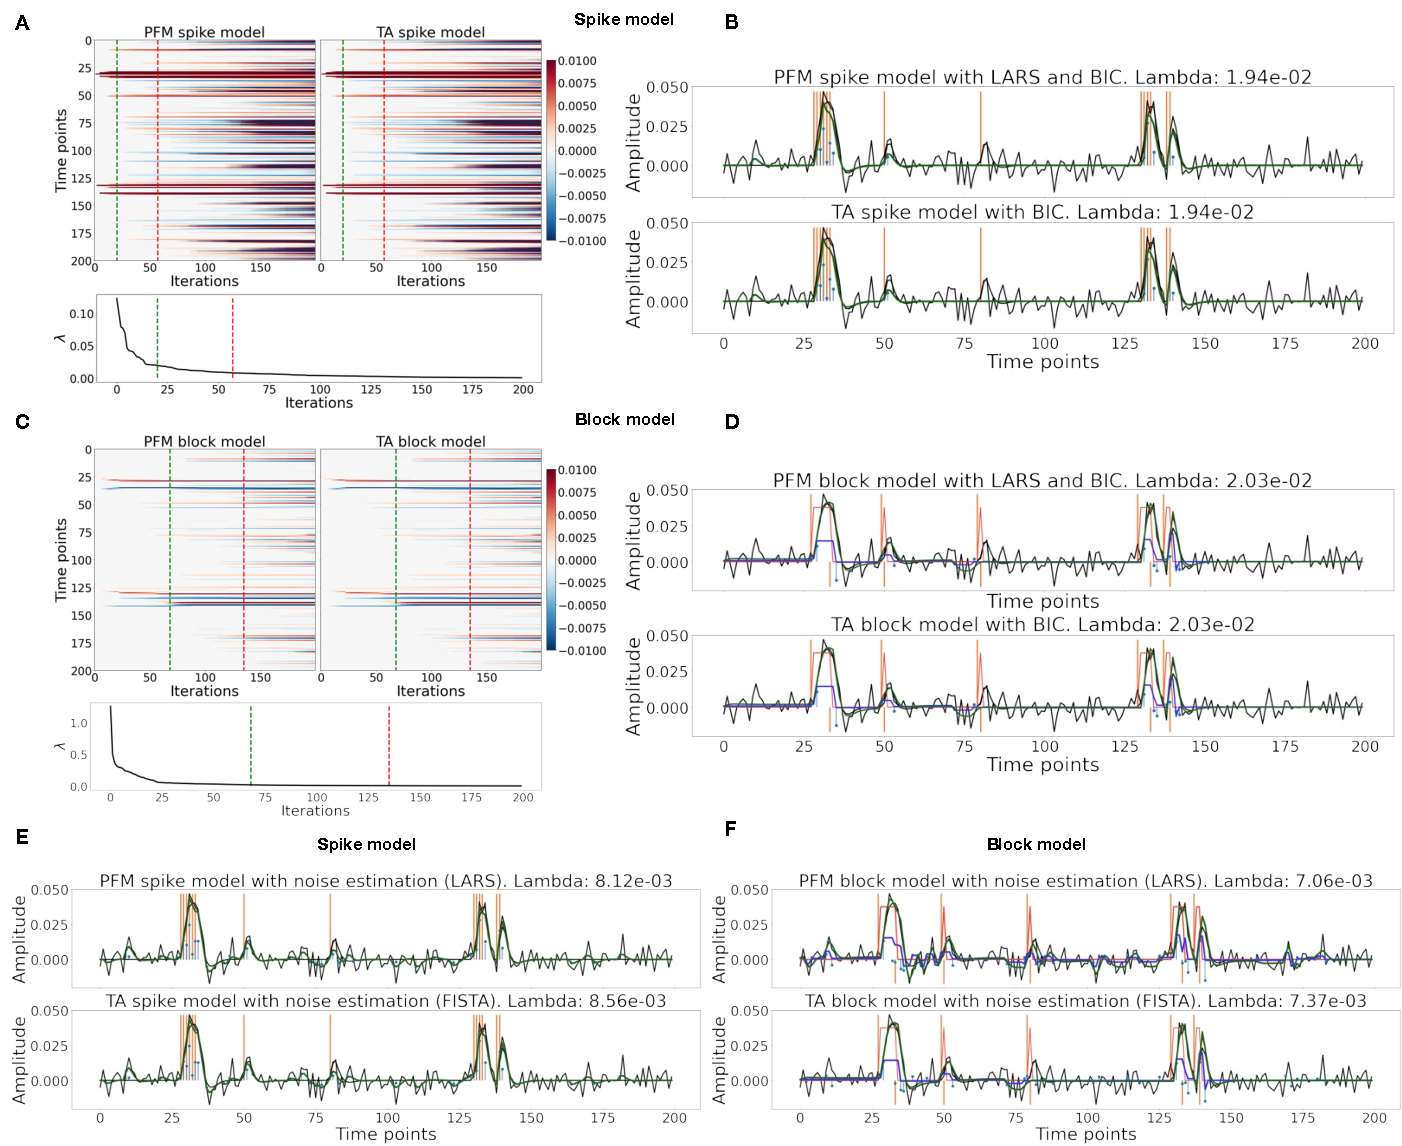
\includegraphics[width=\textwidth]{figures/synthesis_analysis/figure_sim.pdf}
    \end{center}
    \caption{(A) Heatmap of the regularization paths of the activity-inducing
    signals (spike model) estimated with PFM and TA as a function of $\lambda$
    for the simulated data with SNR = 3 dB (x-axis: increasing number of
    iterations or $\lambda$ as given by LARS; y-axis: time; color: amplitude).
    Vertical lines denote iterations corresponding to the BIC (dashed line) and
    MAD (dotted line) selection of $\lambda$. (B) Estimated activity-inducing
    (blue) and activity-related (green) signals with a selection of $\lambda$
    based on the BIC. Orange and red lines depict the ground truth. (C) Heatmap
    of the regularization paths of the innovation signals (block model)
    estimated with PFM and TA as a function of $\lambda$ for the simulated data
    with SNR = 3 dB. (D) Estimated innovation (blue), activity-inducing (darker
    blue), and activity-related (green) signals with a selection of $\lambda$
    based on the BIC. (E) Activity-inducing and activity-related (fit,
    $\mathbf{x}$) signals estimated with PFM (top) and TA (bottom) when
    $\lambda$ is selected based on the MAD method with the spike model, and (F)
    with the block model for the simulated data with SNR = 3 dB.}
\label{fig:sim}
\end{figure}

\subsection{Performance on Experimental Data}

\cref{fig:rss} depicts the \acrshort*{rssd} maps revealing differences between
PFM and TA estimates for the spike (\cref{fig:rss}A and C) and block
(\cref{fig:rss}B and D) models when applied to the three experimental fMRI
datasets. The RSSD values are virtually negligible (i.e., depicted in yellow) in
most of the within-brain voxels and lower than the amplitude of the estimates of
the activity-inducing and innovation signals. Based on the maximum value of the
range shown in each image, it can be observed that the similarity between both
approaches is more evident for the spike model (with both selection criteria)
and the block model with the BIC selection. However, given the different
approaches used for the selection of the regularization parameter $\lambda$
based on the MAD estimate of the noise (i.e., converging so that the residuals
of FISTA are equal to the MAD estimate of the noise for TA vs. finding the LARS
residual that is closest to the MAD estimate of the noise), higher RSSD values
can be observed with the largest differences occurring in gray matter voxels.
These areas also correspond to low values of $\lambda$ (see \cref{fig:lambdas})
and MAD estimates of the noise (see \cref{fig:mad_estimate}), while the highest
values are visible in regions with signal droupouts, ventricles, and white
matter. These differences that arise from the different approaches to find the
optimal regularization parameter based on the MAD estimate of the noise can be
clearly seen in the root sum of squares (RSS) of the estimates
(\cref{fig:rss_comparison}). These differences are also observable in the
\acrshort*{ats} calculated from estimates obtained with the MAD selection as
shown in \cref{fig:task_mad}. However, the identical regularization paths shown
in \cref{fig:motor_regpaths} demonstrate that both methods perform equivalently
on experimental data (see estimates of innovation signal obtained with an
identical selection of $\lambda$ in \cref{fig:mad_inno_ts}). Hence, the higher
RSSD values originate from the different methods to find the optimal
regularization parameter based on the MAD estimate of the noise that yield
different solutions as shown by the dashed vertical lines in
\cref{fig:motor_regpaths}.

\begin{figure}[t!]
    \begin{center}
        \includegraphics[width=\textwidth]{figures/synthesis_analysis/rssd_maps.png}
    \end{center}
    \caption{Square root of the sum of squared differences (RSSD) between the estimates obtained with PFM and TA for (A) spike model (activity-inducing signal) and BIC selection of $\lambda$, (B) block model (innovation signal) and BIC selection, (C) spike model (activity-inducing signal) and MAD selection, (D) block model (innovation signal) and MAD selection. RSSD maps are shown for the three experimental fMRI datasets: the motor task (Motor), the monoband resting-state (Mono), and the multiband resting-state (Multi) datasets.}
\label{fig:rss}
\end{figure}

\cref{fig:task_maps} depicts the results of the analysis of the Motor dataset
with the PFM and TA algorithms using the BIC selection of $\lambda$ (see
\cref{fig:task_mad} for results with MAD selection), as well as a conventional
GLM approach. The Activation Time Series (top left), calculated as the sum of
squares of all voxel amplitudes (positive vs. negative) for a given moment in
time, obtained with PFM and TA show nearly identical patterns. These ATS help to
summarize the four dimensional information available in the results across the
spatial domain and identify instances of significant BOLD activity. The second
to sixth rows show the voxel timeseries and the corresponding activity-related,
activity-inducing and innovation signals obtained with PFM using the BIC
criterion of representative voxels in the regions activated in each of the motor
tasks. The TA-estimated time-series are not shown because they were virtually
identical. The maps shown on the right correspond to statistical parametric maps
obtained with the GLM for each motor condition ($p < 0.001$) as well as the maps
of the PFM and TA estimates at the onsets of individual motor events (indicated
with arrows in the timecourses). The estimated activity-related,
activity-inducing and innovation signals clearly reveal the activity patterns of
each condition in the task, as they exhibit a BOLD response locked to the onset
and duration of the conditions. Overall, activity maps of the innovation signal
obtained with PFM and TA highly resemble those obtained with a GLM for
individual events, with small differences arising from the distinct specificity
of the GLM and deconvolution analyses. Notice that the differences observed with
the different approaches to select $\lambda$ based on the MAD estimate shown in
\cref{fig:rss} are reflected on the ATS shown in \cref{fig:task_mad} as well.

\begin{figure}[t!]
    \begin{center}
        \includegraphics[width=\textwidth]{figures/synthesis_analysis/task_maps.png}
    \end{center}
    \caption{Activity maps of the motor task using a selection of $\lambda$ based on the BIC estimate. Row 1: Activation time-series (ATS) of the innovation signals estimated by PFM (in blue) or TA (in red) calculated as the sum of squares of all voxels at every timepoint. Positive-valued and negative-valued contributions were separated into two distinct time-courses. Color-bands indicate the onset and duration of each condition in the task (green: tongue motion, purple: left-hand finger-tapping, blue: right-hand finger-tapping, red: left-foot toes motion, orange: right-foot toes motion). Rows 2-6: time-series of a representative voxel for each task with the PFM-estimated innovation (blue), PFM-estimated activity-inducing (green), and activity-related (i.e., fitted, orange) signals, with their corresponding GLM, PFM, and TA maps on the right (representative voxels indicated with green arrows). Amplitudes are given in signal percentage change (SPC). The maps shown on the right are sampled at the time-points labeled with the red arrows and display the innovation signals at these moments across the whole brain.}
\label{fig:task_maps}
\end{figure}

As an illustration of the insights that deconvolution methods can provide in the
analysis of resting-state data, \cref{fig:caps} depicts the average
activity-inducing and innovation maps of common resting-state networks obtained
from thresholding and averaging the activity-inducing and innovation signals,
respectively, estimated from the resting-state multiband data using PFM with a
selection of $\lambda$ based on the BIC. The average activity-inducing maps
obtained via deconvolution show spatial patterns of the default mode network
(DMN), dorsal attention network (\acrshort*{dan}), and visual network (VIS) that
highly resemble the maps obtained with conventional seed correlation analysis
using Pearson's correlation, and the average maps of extreme points of the
signal (i.e., with no deconvolution). With deconvolution, the average
activity-inducing maps seem to depict more accurate spatial delineation (i.e.,
less smoothness) than those obtained from the original data, while maintaining
the structure of the networks. The BIC-informed selection of $\lambda$ yields
spatial patterns of average activity-inducing and innovation maps that are more
sparse than those obtained with a selection of $\lambda$ based on the MAD
estimate (see \cref{fig:caps_mad}). Furthermore, the spatial patterns of the
average innovation maps based on the innovation signals using the block model
yield complementary information to those obtained with the activity-inducing
signal since iCAPs allow to reveal regions with synchronous innovations, i.e.,
with the same upregulating and downregulating events. For instance, it is
interesting to observe that the structure of the visual network nearly
disappears in its corresponding average innovation maps, suggesting the
existence of different temporal neuronal patterns across voxels in the primary
and secondary visual cortices.

\begin{figure}[t!]
    \begin{center}
        \includegraphics[width=\textwidth]{figures/synthesis_analysis/caps.png}
    \end{center}
    \caption{Average activity-inducing (left) and innovation (right) maps
    obtained from PFM-estimated activity-inducing and innovation signals,
    respectively, using a BIC-based selection of $\lambda$. Time-points selected
    with a 95\textsuperscript{th} percentile threshold (horizontal lines) are
    shown over the average time-series (blue) in the seed region (white cross)
    and the deconvolved signals, i.e., activity inducing (left) and innovation
    (right) signals (orange). Average maps of extreme points and seed
    correlation maps are illustrated in the center.}
\label{fig:caps}
\end{figure}

% Discussion
\section{Discussion and Conclusion}
\label{sec:synthesis_discussion}

Hemodynamic deconvolution can be formulated using a synthesis- and
analysis-based approach as proposed by PFM and TA, respectively. This work
demonstrates that the theoretical equivalence of both approaches is confirmed in
practice given virtually identical results when the same HRF model and
equivalent regularization parameters are employed. Hence, it can be argued that
previously observed differences in performance can be explained by specific
settings, such as the HRF model and selection of the regularization parameter
(as shown in \cref{fig:rss,fig:rss_comparison,fig:motor_regpaths}), convergence
thresholds, as well as the addition of a spatial regularization term in the
spatiotemporal TA formulation \citep{Karahanoglu2013TotalactivationfMRI}. For
instance, the use of PFM with the spike model in
\cite{Tan2017DecodingfMRIevents} was seen not to be adequate due to the
prolonged trials in the paradigm, which better fit the block model as described
in \cref{eq:pfm_block}. However, given the equivalence of the temporal
deconvolution, incorporating extra spatial or temporal regularization terms in
the optimization problem should not modify this equivalence providing convex
operators are employed. For a convex optimization problem, with a unique global
solution, iterative shrinkage thresholding procedures alternating between the
different regularization terms guarantee convergence, such as the generalized
forward-backward splitting \citep{Raguet2013GeneralizedForwardBackward}
algorithm originally employed for TA. 

Our findings are also in line with the equivalence of analysis and synthesis
methods in under-determined cases (\(N \leq V\)) demonstrated in
\citep{Elad2007Analysisversussynthesis} and
\citep{Ortelli2019Synthesisanalysistotal}. Still, this chapter has shown that a
slight difference in the selection of the regularization parameter can lead to
small differences in the estimated signals when employing the block model with
the \acrshort*{bic} selection of $\lambda$. However, since their regularization
paths are equivalent, the algorithms can easily be forced to converge to the
same selection of $\lambda$, thus resulting in identical estimated signals.

Nevertheless, the different formulations of analysis and synthesis deconvolution
models bring along different kinds of flexibility. One notable advantage of PFM
is that it can readily incorporate any HRF as part of the synthesis operator
\citep{Elad2007Analysisversussynthesis}, only requiring the sampled HRF at the
desired temporal resolution, which is typically equal to the TR of the
acquisition. Conversely, TA relies upon the specification of the discrete
differential operator that inverts the HRF, which needs to be derived either by
the inverse solution of the sampled HRF impulse response, or by discretizing a
continuous-domain differential operator motivated by a biophysical model. The
more versatile structure of PFM allows for instance an elegant extension of the
algorithm to multi-echo fMRI data
\citep{CaballeroGaudes2019deconvolutionalgorithmmulti} where multiple
measurements relate to a common underlying signal. Therefore, the one-to-many
synthesis scenario (i.e., from activity-inducing to several activity-related
signals) is more cumbersome to express using TA. In other words, a set of
differential operators should be defined and the differences between their
outputs constrained. In contrast, the one-to-many analysis scenario (i.e., from
the measurements to several regularizing signals) is more convenient to be
expressed by TA, for example combining spike and block regularizers. While the
specification of the differential operator in TA only indirectly controls the
HRF, the use of the derivative operator to enforce the block model, instead of
the integrator in PFM, impacts positively the stability and rate of the
convergence of the optimization algorithms. Moreover, analysis formulations can
be more suitable for online applications that are still to be explored in fMRI
data, but are employed for calcium imaging deconvolution
\citep{Friedrich2017Fastonlinedeconvolution,Jewell2019Fastnonconvexdeconvolution},
and which have been applied for offline calcium deconvolution
\citep{Farouj2020DeconvolutionSustainedNeural}.

Moreover, deconvolution techniques can be used before more downstream analysis
of brain activity in terms of functional network organization as they estimate
interactions between voxels or brain regions that occur at the activity-inducing
level, and are thus less affected by the slowness of the hemodynamic response
compared to when the BOLD signals are analyzed directly. In particular,
hemodynamic deconvolution approaches hold a close parallelism to recent
methodologies aiming to understand the dynamics of neuronal activations and
interactions at short temporal resolution and that focus on extreme events of
the fMRI signal. As an illustration, \cref{fig:caps} shows that the innovation-
or activity-inducing CAPs computed from deconvolved events in a single
resting-state fMRI dataset closely resemble the conventional CAPs computed
directly from extreme events of the fMRI signal
\citep{Liu2013Timevaryingfunctional,Liu2013Decompositionspontaneousbrain,
Liu2018Coactivationpatterns,Cifre2020Revisitingnonlinear,Cifre2020Furtherresultswhy,
Zhang2020relationshipBOLDneural,Tagliazucchi2011SpontaneousBOLDevent,Tagliazucchi2012Criticalitylargescale,
Tagliazucchi2016VoxelWiseFunctional,Rolls2021BraindynamicsSynchronous}.
Similarly, it can be hypothesized that these extreme events will also show a
close resemblance to intrinsic ignition events
\citep{Deco2017HierarchyInformationProcessing,Deco2017NovelIntrinsicIgnition}.
As shown in the maps, deconvolution approaches can offer a more straightforward
interpretability of the activation events and resulting functional connectivity
patterns. Here, CAPs were computed as the average of spatial maps corresponding
to the events of a single dataset. Beyond simple averaging, clustering
algorithms (e.g., K-means and consensus clustering) can be employed to discern
multiple CAPs or iCAPs at the whole-brain level for a large number of subjects.
Previous findings based on iCAPs have for instance revealed organizational
principles of brain function during rest
\citep{Karahanoglu2015Transientbrainactivity} and sleep
\citep{Tarun2021NREMsleepstages} in healthy controls, next to alterations in
22q11ds \citep{Zoeller2019LargeScaleBrain} and multiple sclerosis
\citep{Bommarito2021Alteredanteriordefault}. 

Next to CAPs-inspired approaches, dynamic functional connectivity has recently
been investigated with the use of co-fluctuations and edge-centric techniques
\citep{Faskowitz2020Edgecentricfunctional,Esfahlani2020Highamplitudecofluctuations,Jo2021Subjectidentificationusing,Sporns2021Dynamicexpressionbrain,Oort2018Functionalparcellationusing}.
The activation time series shown in \cref{fig:task_maps}A aims to provide
equivalent information to the root of sum of squares timecourses used in
edge-centric approaches, where timecourses with peaks delineate instances of
significant brain activity. Future work could address which type of information
is redundant or distinct across these frameworks. These examples illustrate that
deconvolution techniques can be employed prior to other computational approaches
and could serve as an effective way of denoising the fMRI data. Hence, an
increase in the number of studies that take advantage of the potential benefits
of using deconvolution methods prior to functional connectivity analyses can be
expected.

Even though the two approaches examined here provide alternative representations
of the BOLD signals in terms of innovation and activity-inducing signals, their
current implementations have certain limitations and call for further
developments or more elaborate models, where some of them have been partially
addressed in the literature. One relevant focus is to account for the
variability in HRF that can be observed in different regions of the brain.
First, variability in the temporal characteristics of the HRF can arise from
differences in stimulus intensity and patterns, as well as with short
inter-event intervals like in fast cognitive processes or experimental designs
\citep{Yesilyurt2008DynamicsnonlinearitiesBOLD,
Sadaghiani2009Neuralactivityinduced,Chen2021Investigatingmechanismsfast,Polimeni2021Imagingfasterneural}.
Similarly, the HRF shape at rest might differ from the canonical HRF commonly
used for task-based fMRI data analysis. A wide variety of HRF patterns could be
elicited across the whole brain and possible detected with sufficiently large
signal-to-noise ratio. For instance, \cite{GonzalezCastillo2012Wholebraintime}
showed two gamma-shaped responses at the onset and the end of the evoked trial,
respectively. This unique HRF shape would be deconvolved as two separate events
with the conventional deconvolution techniques. The impact of HRF variability
could be reduced using structured regularization terms along with multiple basis
functions \citep{Gaudes2012Structuredsparsedeconvolution} or procedures that
estimate the HRF shape in an adaptive fashion in both analysis
\citep{Farouj2019BoldSignalDeconvolution} and synthesis formulations
\citep{Cherkaoui2021Multivariatesemiblind}.

Another avenue of research consists in leveraging spatial information by
adopting multivariate deconvolution approaches that operate at the whole-brain
level, instead of working voxelwise and beyond regional regularization terms
(e.g., as proposed in \cite{Karahanoglu2013TotalactivationfMRI}). Operating at
the whole-brain level would open the way for methods that consider shared
neuronal activity using mixed norm regularization terms
\citep{UrunuelaTremino2019Deconvolutionmultiecho}, as described in
\cref{cha:multivariate}, or can capture long-range neuronal cofluctuations using
low rank decompositions \citep{Cherkaoui2021Multivariatesemiblind}. For example,
multivariate deconvolution approaches could yield better localized activity
patterns while reducing the effect of global fluctuations such as respiratory
artifacts, which cannot be modelled at the voxel level with a multivariate
sparse and low-rank model \citep{Urunuela2021LowRankSparse}, as described in
\cref{cha:low-rank}.

Similar to solving other inverse problems by means of regularized estimators,
the selection of the regularization parameter is critical to correctly estimate
the neuronal-related signal. Hence, methods that take advantage of a more robust
selection of the regularization parameter could considerably yield more reliable
estimates of the neuronal-related signal. For instance, the stability selection
procedure
\citep{Meinshausen2010Stabilityselection,Urunuela2020StabilityBasedSparse}could
be included to the deconvolution problem to ensure that the estimated
coefficients are obtained with high probability. This approach is described in
\cref{cha:stability} \citep{Urunuela2020StabilityBasedSparse}. Furthermore, an
important issue of regularized estimation is that the estimates are biased with
respect to the true value. In that sense, the use of non-convex
\(\ell_{p,q}\)-norm regularization terms (e.g., \(p < 1\)) can reduce this bias
while maintaining the sparsity constraint, at the cost of potentially converging
to a local minima of the regularized estimation problem. In practice, these
approaches could avoid the optional debiasing step that overcomes the shrinkage
of the estimates and obtain a more accurate and less biased fit of the fMRI
signal
\citep{Gaudes2013Paradigmfreemapping,CaballeroGaudes2019deconvolutionalgorithmmulti}.
Finally, cutting-edge developments on physics-informed deep learning techniques
for inverse problems
\citep{Akcakaya2021UnsupervisedDeepLearning,Monga2021AlgorithmUnrollingInterpretable,Ongie2020DeepLearningTechniques,Cherkaoui2020LearningsolveTV}
could be transferred for deconvolution by considering the biophysical model of
the hemodynamic system and could potentially offer algorithms with reduced
computational time and more flexibility.

\section{Code and data availability}
\label{sec:synthesis_github}
The code and materials used in this work can be found in the following GitHub
repository: \url{https://github.com/eurunuela/pfm_vs_ta}. The reader can explore
different simulation parameters (e.g., SNR, varying HRF options and mismatch
between algorithms, TR, number of events, onsets, and durations) in the provided
Jupyter notebooks. Similarly, the experimental data can be found in
\url{https://osf.io/f3ryg/}.